% Template PNSAC newsletter - Article
% Language: Latex
%

% Head

\title{Volunteers Assure a Bright Future for Classic Plane}
%\subtitle{Part 4}
\author{Randall Denley}

\maketitle

\end{multicols}

\begin{figure*}[htbp]
	\vspace{2em}
	\centering
	%name of the graphic, without the path AND in EPS format:
	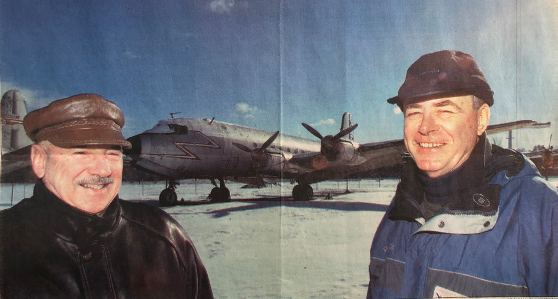
\includegraphics[scale=0.8]{holmgren-timmin-scaled.png}
	%caption of the figure 
	\caption*{\small \em TIm Timmins, left, and Robert Holmgren are forming a
group of skilled volunteers to restore a 55-year-old North Star, the first
Canadian-made plane capable of transcontinental flight.}
	%label of the figure, which has to correspond to \ref{}:
	\label{fig:timmins-holmgren}
\end{figure*}


\begin{multicols}{2}

\textit{This article was published in the Ottawa Citizen on February 1, 2003
under the byline of Randall Denley. It was brought to our attention recently by
Drew Hodge. The article is republished with the express permission of the
Ottawa Citizen, a division of Postmedia Network Inc. (ed.).
}\\

The world's last classic Canadair North Star sits, forlorn, on the tarmac at
the Canada Aviation Museum. It's been parked there since 1966, along with half
a dozen other orphans of the museum, planes that it has no money to restore and
that are too big to bring inside the crowded building.

The paint on the North Star is faded and peeling.Some gaps in the wings are
closed with wire to keep out the birds that have made it home for years.The
engines are protected with pieces of plywood. The interior requires a complete
renovation.

It's a shame to see an important part of Canada's aviation history slide into
this kind of ruin, Thanks to the efforts of two Ottawa men, however, the North
Star finally has a bright future.

Robert Holmgren and Tim Timmins are forming a group of skilled volunteers to
restore the North Star. This kind of volunteer effort will be a first for the
museum, says director general Anthony Smyth, who is supporting the effort,
along with aviation companies including Air Canada and Boeing.

The museum is showing commendable flexibility because the traditional view in
the museum world is that restoration is work that can only be done by trained
experts. Unfortunately, the museum can't afford that kind of work, and that's
one of the reasons the plane has been sitting there for more than 35 years.

This is no small undertaking. The 55-year-old North Star 1-ST is a sizeable
plane, nearly 30 metres long and with a wing span of 35 metres. Restoring it
will be a yearlong process that would cost \$1 million if it were done by paid
staff.

The North Star is an important plane in Canada's aviation history, the first
Canadian-,made plane capable of transcontinental flight. It's considered the
plane that launched the postwar Canadian aviation industry; 70 of them were
built. Brought into service after the Second World War, North Stars carried
passengers for several airlines and troops for the Canadian military.  North
Stars served to airlift Canadian troops to Korea and provided transportation
for VIPs visiting Canada. The plane at the museum belonged to the RCAF.

Holmgren is a retired Air Canada maintenance expert, and Timmins is a former
RCAF navigator who flew on the North Stars. Timmins's former squadron had taken
an interest in the North Star, and Holmgren, who was giving his time as a
volunteer at the museum, pushed it forward.

"We'd like to see it brought back to something like its former self," Holmgren
says.

A temporary structure, perhaps a bubble like the one over the playing field at
Lansdowne Park, will be necessary before the restoration can begin. The plane
is too large to fit inside the museum's existing building and also too big to
be easily transported elsewhere.

Holmgren and Timmins need about 200 volunteers to make the project a success.
Holmgren has approached Air Canada, Bombardier and Boeing to get the help of
past and present employees. About 40 volunteers have already come forward.

The key need is skilled craftsmen with up-to-date large aircraft experience and
who live in or near Ottawa.

Some people who can come in almost every day to run the project are required. 
There is also a demand for people to do record-keeping and research.

The group is hoping to attract national attention for the project, both to
provide volunteer expertise and to help raise money.  This is a plan to help a
national museum, after all.  Smyth says the museum will be involved with a
fundraising campaign, but it's early yet to say how much is required. It
depends partly on how much time and material are donated by corporations. A
full-time salaried project manager will be hired by the museum.

The project will take a conservation approach, retaining as much of the
original material as possible, Smyth says. The restored plane will be
structurally complete and faithful to the original. Returning the plane to
flyable condition is too expensive to be feasible and the museum wouldn't want
to take a chance flying the last remaining version of such an important plane.

Restoring the North Star is just the beginning of what Holmgren and his
associates hope to accomplish. The museum has another half dozen planes outside
that require restoration. Restoring them all will take nine or ten years. The
Museum's new addition, which it hopes to have open by December of this year,
will be large enough to finally bring the North Star indoors.

%If you want to help with the project, contact Robert Holmgren at 748-5972 or
%robertholmgren@rogers.com. The group also has a Web site,
%www.projectnorthstar.ca.

%\address{Web site:
%{\normalfont\color{blue}\texttt{\url{http://www.projectnorthstar.ca}}}\\
%	General enquiries:\email{info@projectnorthstar.ca}}
%


%\begin{quotation}
%	\textit{You have to be careful opening up the panels covering the 
%	engines, you never know if a bird or some animal might have made
%	its home there.}
%\end{quotation}

%\begin{figure*}[htbp]
%	\vspace{2em}
%	\centering
%	%name of the graphic, without the path AND in EPS format:
%	\includegraphics[scale=0.5]{op-hawk-one.jpg}
%	%caption of the figure 
%	%\caption*{\small \em Volunteers put in countless hours restoring a
%	North Star aircraft.}
%	%label of the figure, which has to correspond to \ref{}:
%	\label{fig:op-hawk-one.eps}
%\end{figure*}


\begin{footnotesize}
    \raggedleft PNSAC\\
\end{footnotesize}

% End of text.

%%% Local Variables: 
%%% mode: latex
%%% TeX-master: main_document.tex
%%% End: 

